\documentclass[a4paper,12pt]{report}

\usepackage{cmap}
\usepackage[T2A]{fontenc}
\usepackage[utf8]{inputenc}
\usepackage[russian]{babel}
\usepackage{amsmath,amsfonts,amssymb}
\usepackage{graphicx}
\usepackage{sidecap}
\usepackage{wrapfig}
\usepackage{indentfirst}

\begin{document} 

\begin{titlepage} 

\begin{center} 

\large Федеральное государственное автономное образовательное учреждение высшего образования «Санкт-Петербургский государственный электротехнический университет «ЛЭТИ» им. В.И. Ульянова (Ленина)»\\
кафедра Вычислительной техники\\[5cm] 

\huge ОТЧЕТ\\ по лабораторной работе № 9\\[0.5cm] 
\large <<Линейные двусвязные списки>>\\[3.7cm]

\begin{minipage}{1\textwidth}
    \begin{flushleft}
        \emph{Автор:} Стукен В.А.\\
        \emph{Группа:} 2307\\
        \emph{Факультет:} ФКТИ\\
        \emph{Преподаватель:} Аббас Саддам Ахмед\\
    \end{flushleft}
\end{minipage}

\vfill

Санкт-Петербург, 2023\\
{\large \LaTeX}

\end{center}
\thispagestyle{empty}
\end{titlepage}

\section*{Задание(вариант 3)}
Разработать подалгоритм и написать функцию, удаляющую в двусвязном списке заданный по номеру элемент. Номер элемента задается с конца списка. При недостаточном количестве элементов в списке удалить элемент из начала списка (первый). При пустом списке вывести соответствующее сообщение.
\section*{Постановка задачи и описание решения}
\par

Сначала задаем двусвязный список производителей с помощью ф-ции $create_Dlist()$, она возвращает голову этого списка.
Затем с помощью ф-ции $select_by_manuf()$ добавляем в поля элементов односвязного списка указатели на соответствующие элементы двусвязного списка.
Выводим исходный список. 
Далее просим пользователя ввести номер двусвязного списка, который надо удалить. Далее ищем этот элемент в списке с помощью ф-ции $Dselect_by_id()$ и удаляем этот элемент с помощью ф-ции $deleteNode()$
Выводим полученный список.

\section*{Описание переменных-функция main}
\begin{centering}
\resizebox{14cm}{!}{
    \begin{tabular}{|l|l|l|l|}
        \hline
        \textbf{№} & \textbf{Имя переменной} & \textbf{Тип} & \textbf{Назначение}\\
        \hline
        1 & fp         &FILE*& Указатель на файл\\ 
        \hline
        2 &  S,S0           & Node*  & Указатели на узлы списка\\ 
        \hline
        3 &  H   &  Head* & Указатель на голову односвязного списка \\
        \hline
        4 & s1        & char[] & Строка файла\\ 
        \hline
        5 & s2           & char[][] & Двумерный массив строк \\
        \hline
        6 & slen    & int & Длина строки \\
        \hline
        7 & number    & int & Id элемента \\
        \hline
        8 & position   & int & Позиция, куда надо скопировать эл. \\
        \hline
        9 & target-node   & Node* & Указатель на элемент с указанным id\\
        \hline
        10 & node-after & Node* & Указатель на элемент на определенной позиции \\
        \hline
        11 & head*   &  DHead* & Указатель на голову двусвязного списка \\
        \hline
        12 & found   &  DNode* & Указатель на найденный элемент двусвязного списка \\
        \hline
    \end{tabular}
}
\end{centering}
\section*{Примеры работы программы:}
\begin{figure}[ph]
    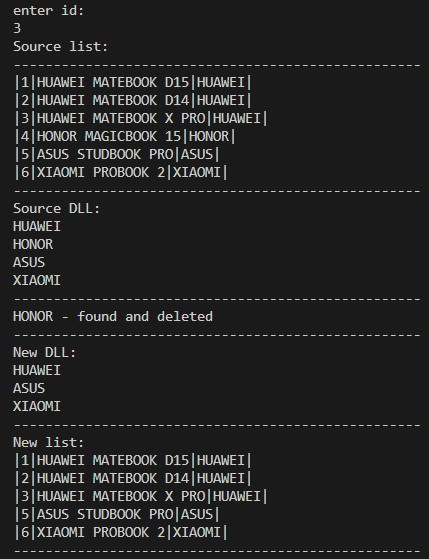
\includegraphics[width=0.6\textwidth]{ex1.jpg}
\caption{Пример 1}
\label{ris:image1}
    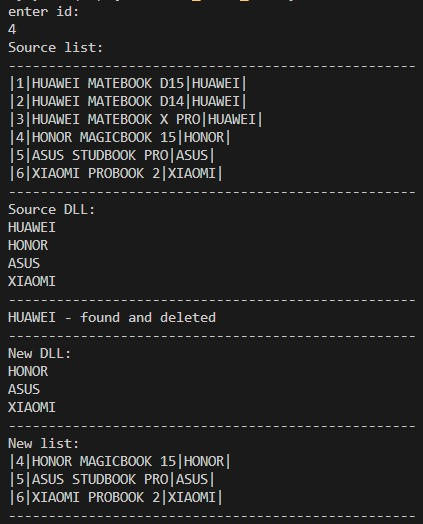
\includegraphics[width=0.7\textwidth]{ex2.jpg}
\caption{Пример 2}
\label{ris:image2}


\end{figure}

\begin{figure}[ph]
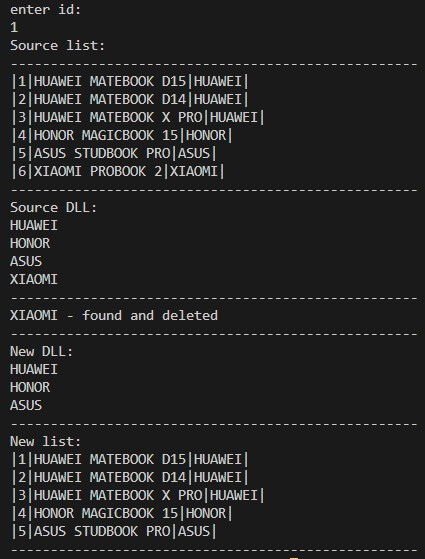
\includegraphics[width=0.7\textwidth]{ex3.jpg}
\caption{Пример 3}
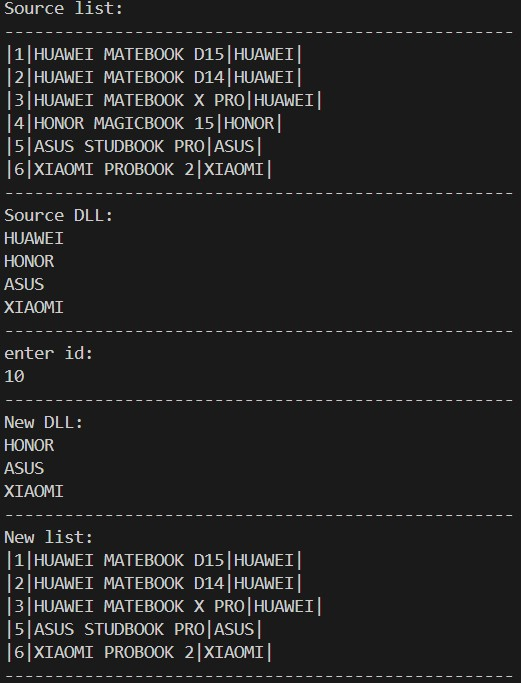
\includegraphics[width=0.7\textwidth]{ex4.jpg}
\caption{Пример 4}
\label{ris:image3}

\end{figure}


\newpage

\section*{Вывод}
В данной лабораторной работе научились работать с двусвязными списками в языке Си, 
реализовали простейший алгоритм удаления элемента двусвязного списка.
\end{document}